\section{Devise a way to parallelize} \label{s:general-approach:devise-a-way-to-parallelize}
	This section introduces ways of parallelization three numerical methods: \emph{explicit upwind}, \emph{implicit upwind} and \emph{Crank-Nicolson}. Each of them contains figure in a subsection describing the task division in domain of time and space. Second figure for all schemes will present parallelism of work by processors. Following subsections refer to \gls{stencil}s of numerical methods in order to extract necessary data to send between processors. Figure \ref{fig:visualization:serial-calculations} bases on Figure \ref{fig:schematicOfFDM} and shows the data flow during calculations of next time steps using serial algorithm. Additionally mentioned figure constitute to parallel visualizations In each time step values in the grid are closer (opacity of green color) to the desired values. All the calculations are performed by a single processor for each point in the grid. After reaching certain time step calculations are stopped. 
	\begin{figure}[!htbp]
		\centering
		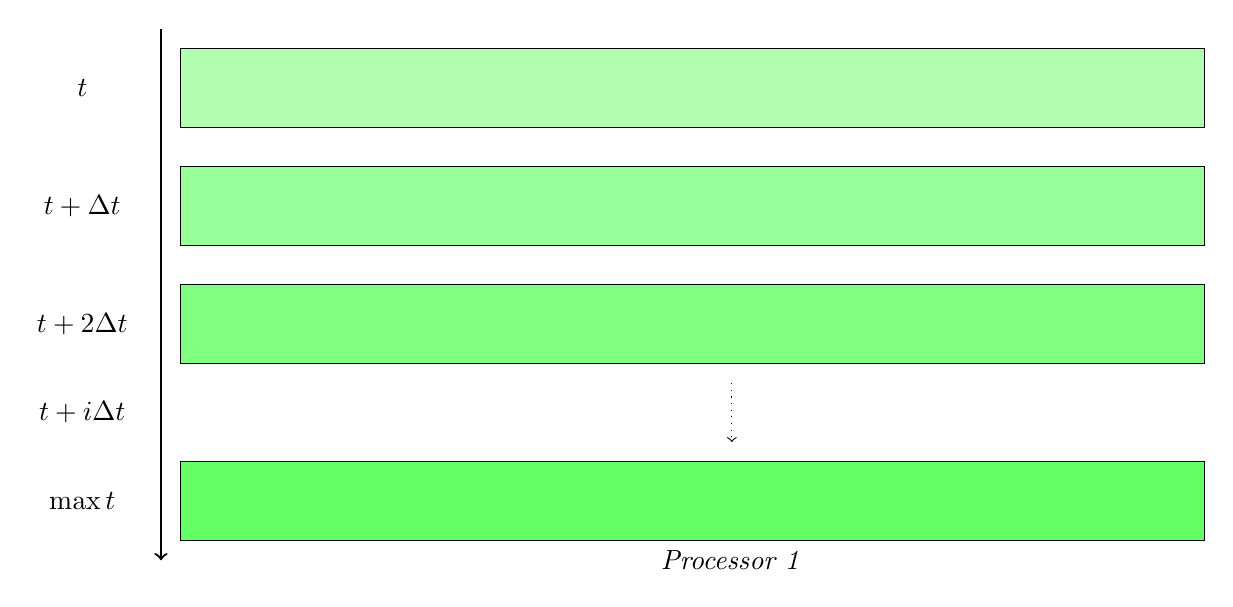
\begin{tikzpicture}[scale=1.0]
			\draw [->] [black, thick] (-.25, 0.25) -- (-.25, -6.5);
			\filldraw[fill=green!30!white, draw=black] (0,0) rectangle (13,-1);
			\node[black] at (-1.25, -0.5) {$t$};
			\filldraw[fill=green!40!white, draw=black] (0,-1.5) rectangle (13,-2.5);
			\node[black] at (-1.25, -2) {$t + \Delta t$};
			\filldraw[fill=green!50!white, draw=black] (0,-3) rectangle (13,-4);
			\node[black] at (-1.25, -3.5) {$t + 2\Delta t$};
			\draw [->] [dotted] (7, -4.25) -- (7, -5);
			\node[black] at (-1.25, -4.25 - 0.75/2) {$t + i \Delta t$};
			\filldraw[fill=green!60!white, draw=black] (0,-5.25) rectangle (13,-6.25);
			\node[black] at (-1.25, -5.75) {$\max t$};
			\node[black] at (7, -6.5) {\emph{Processor 1}};
		\end{tikzpicture}
		\caption{Visualization of serial calculations for one dimensional grid.}
		\label{fig:visualization:serial-calculations}
	\end{figure}
	
	Considering \gls{stencil}s from all three schemes it is easy to deduct that parallelism at the time has no sense, because solution for next time step always depends on previous and sometimes (for implicit schemes) current solution. However a good idea is to split jobs at the space domain. Spreading grid to local grids among all the processors requires an algorithm to deal with uneven division of grid size and total number of processors. Listing \ref{lst:fragmentation} presents simple algorithm that calculates fragmentation of grid size depending on identification of core and total quantity of cores.
	\begin{lstlisting}[caption=test, label=lst:fragmentation] 
long fragmentation(long coreId, long coresQuantity, long jobSize)
{
	if (coresQuantity == 1)
		return jobSize;
	else if (jobSize % coresQuantity == 0)
		return jobSize / coresQuantity;
	else
	{
		if (coreId == coresQuantity - 1)
			return jobSize / coresQuantity + jobSize % coresQuantity;
		else
			return jobSize / coresQuantity;
	}
}
	\end{lstlisting} 
	It is easy to observe that in this approach last processors will do additional work, which can be in the worst case will be the size of equal to sum modulo of grid size and total quantity of processors (nearly two times more). Since data is stored and spreaded across all processors the second common part of the algorithm is gathering the final results, which requires serial approach. All but main core are obligated to send their local grids to main core in ascending order of core id. Complexity of this problem is of order $\mathcal{O}(n)$, where $n$ is a size of the grid.
	
	\subsection{Explicit upwind scheme parallel algorithm} \label{s:general-approach:explicit-upwind-parallel-algorithm}
	Dependency of the explicit upwind scheme is presented in Figure \ref{fig:stencil:explicit-upwind}. According to the \gls{stencil} in order to calculate new point at time $n+1$ this scheme requires previous and current point of a grid from time $n$. It means that each of the processors requires one value from previous processor (in terms of their ids) to start calculations. Figure \ref{fig:communication:explicit-upwind} presents discussed earlier communication between processors. Transfered $f_{lmax}^{n}$ relates to the last point in the local grid, where $lmax$ is calculated as shown in Listing \ref{lst:fragmentation}.
	\begin{figure}[!htbp]
		\centering
		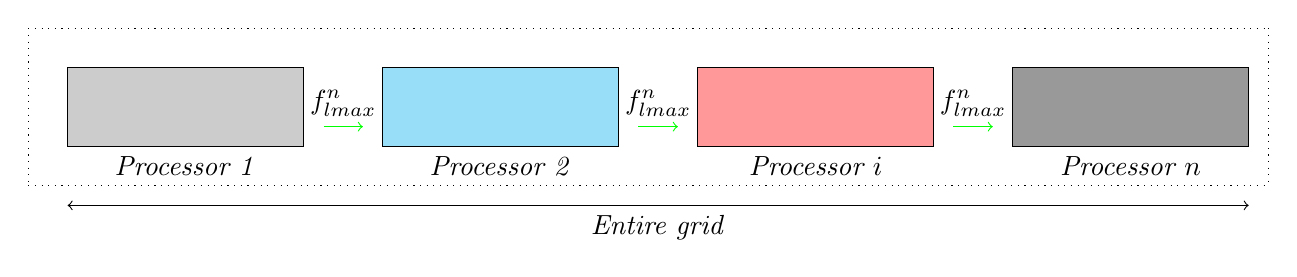
\begin{tikzpicture}[scale=1.0]
			\draw[dotted] (-0.5,-0.5) -- (15.25,-0.5);
			\draw[dotted] (-0.5, 1.5) -- (15.25, 1.5);
			\draw[dotted] (-0.5, 1.5) -- (-0.5, -0.5);
			\draw[dotted] (15.25, 1.5) -- (15.25, -0.5);
			\filldraw[fill=gray!40!white, draw=black] (0,0) rectangle (3,1);
			\filldraw[fill=cyan!40!white, draw=black] (4,0) rectangle (7,1);
			\filldraw[fill=red!40!white, draw=black] (8,0) rectangle (11,1);
			\filldraw[fill=black!40!white, draw=black] (12,0) rectangle (15,1);
			\node[align=right] at (1.5, -0.25) {\emph{Processor 1}};
			\node[align=right] at (5.5, -0.25) {\emph{Processor 2}};
			\node[align=right] at (9.5, -0.25) {\emph{Processor $i$}};
			\node[align=right] at (13.5, -0.25) {\emph{Processor $n$}};
			\draw [->][green] (3.25, 0.25) -- node [midway, above, sloped, black] {$f_{lmax}^{n}$} (3.75, 0.25);
			\draw [->][green] (7.25, 0.25) -- node [midway, above, sloped, black] {$f_{lmax}^{n}$} (7.75, 0.25);
			\draw [->][green] (11.25, 0.25) -- node [midway, above, sloped, black] {$f_{lmax}^{n}$} (11.75, 0.25);
			\draw[<->] (0,-0.75) -- node [midway, below, sloped, black] {\emph{Entire grid}} (15,-0.75);
		\end{tikzpicture}
		\caption{Communication between processors in parallel explicit upwind schema.}
		\label{fig:communication:explicit-upwind}
	\end{figure}
	Parallel calculations for explicit upwind schema are visualized in Figure \ref{fig:visualization:explicit-upwind}. This scheme depends only on current solution so boundary values can be send between neighboring processors before each full iteration through local grids. We can assume that all the processors will be working simultaneously with a small advantage of first processor, because it doesn't have to receive boundary condition. 
	\begin{figure}[!htbp]
		\centering
		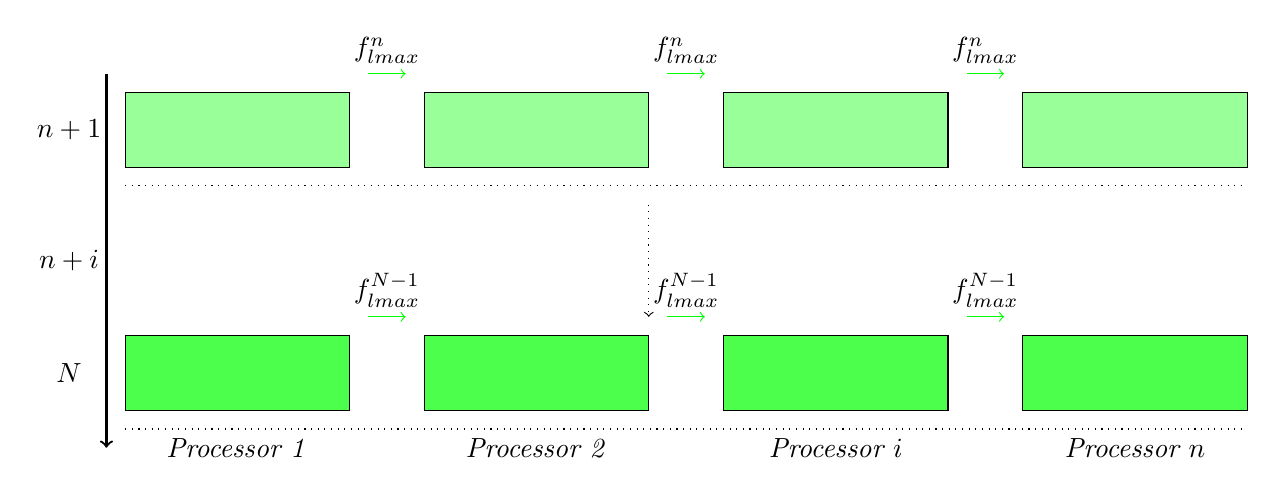
\begin{tikzpicture}[scale=0.95]
			\draw [->] [black, thick] (-.25, 0.25) -- (-.25, -4.75);
			\node[black] at (-0.75, -0.5) {$n+1$};
			\draw [->][green] (3.25, 0.25) -- node [midway, above, sloped, black] {$f_{lmax}^{n}$} (3.75, 0.25);
			\draw [->][green] (7.25, 0.25) -- node [midway, above, sloped, black] {$f_{lmax}^{n}$} (7.75, 0.25);
			\draw [->][green] (11.25, 0.25) -- node [midway, above, sloped, black] {$f_{lmax}^{n}$} (11.75, 0.25);
			\filldraw[fill=green!40!white, draw=black] (0,0) rectangle (3,-1);
			\filldraw[fill=green!40!white, draw=black] (4,0) rectangle (7,-1);
			\filldraw[fill=green!40!white, draw=black] (8,0) rectangle (11,-1);
			\filldraw[fill=green!40!white, draw=black] (12,0) rectangle (15,-1);
			\draw [dotted] (0,-1.25) -- (15,-1.25);
			
			\draw [->] [dotted] (7, -1.5) -- (7, -3);
			
			\node[black] at (-0.75, -2.25) {$n + i$};
			
			\node[black] at (-0.75, -3.75) {$N$};
			\draw [->][green] (3.25, -3) -- node [midway, above, sloped, black] {$f_{lmax}^{N -1}$} (3.75, -3);
			\draw [->][green] (7.25, -3) -- node [midway, above, sloped, black] {$f_{lmax}^{N -1}$} (7.75, -3);
			\draw [->][green] (11.25, -3) -- node [midway, above, sloped, black] {$f_{lmax}^{N -1}$} (11.75, -3);
			\filldraw[fill=green!70!white, draw=black] (0,-3.25) rectangle (3,-4.25);
			\filldraw[fill=green!70!white, draw=black] (4,-3.25) rectangle (7,-4.25);
			\filldraw[fill=green!70!white, draw=black] (8,-3.25) rectangle (11,-4.25);
			\filldraw[fill=green!70!white, draw=black] (12,-3.25) rectangle (15,-4.25);
			\draw [dotted] (0,-4.5) -- (15,-4.5);
			
			\node[align=right] at (1.5, -4.75) {\emph{Processor 1}};
			\node[align=right] at (5.5, -4.75) {\emph{Processor 2}};
			\node[align=right] at (9.5, -4.75) {\emph{Processor $i$}};
			\node[align=right] at (13.5, -4.75) {\emph{Processor $n$}};
			
		\end{tikzpicture}
		\caption{Visualization of parallel calculations for explicit upwind scheme.}
		\label{fig:visualization:explicit-upwind}
	\end{figure}
	\subsection{Implicit upwind scheme parallel algorithm} \label{s:general-approach:implicit-upwind-parallel-algorithm}
	Implicit upwind scheme dependencies are shown in Figure \ref{fig:stencil:implicit-upwind}. According to the \gls{stencil} in order to calculate new point at time $n+1$ this scheme requires previous or next (depending on sign of \gls{CFL}) point of a grid from time $n+1$ and current point at time $n$. It means that each of the processors requires one value from previous processor (in terms of their ids) to start calculations. Figure \ref{fig:communication:implicit-upwind} presents discussed earlier communication between processors. Transfered $f_{lmax}^{n+1}$ relates to the last point in the local grid calculated at time $n+1$, where $lmax$ is determined as shown in Listing \ref{lst:fragmentation}.
	\begin{figure}[!htbp]
		\centering
		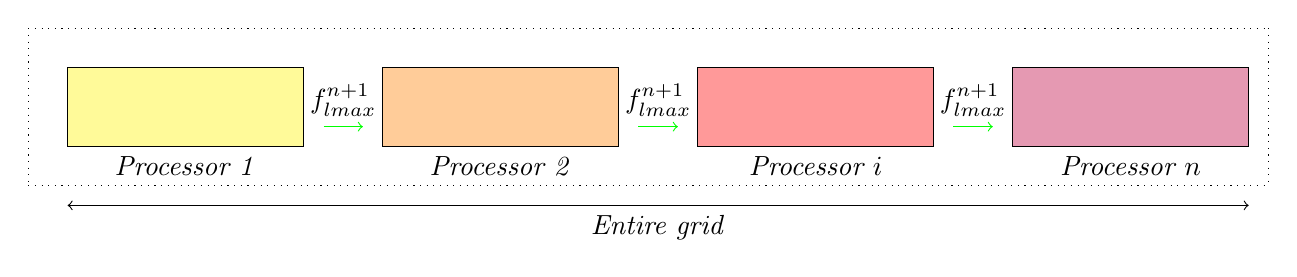
\begin{tikzpicture}[scale=1.0]
			\draw[dotted] (-0.5,-0.5) -- (15.25,-0.5);
			\draw[dotted] (-0.5, 1.5) -- (15.25, 1.5);
			\draw[dotted] (-0.5, 1.5) -- (-0.5, -0.5);
			\draw[dotted] (15.25, 1.5) -- (15.25, -0.5);
			\filldraw[fill=yellow!40!white, draw=black] (0,0) rectangle (3,1);
			\filldraw[fill=orange!40!white, draw=black] (4,0) rectangle (7,1);
			\filldraw[fill=red!40!white, draw=black] (8,0) rectangle (11,1);
			\filldraw[fill=purple!40!white, draw=black] (12,0) rectangle (15,1);
			\node[align=right] at (1.5, -0.25) {\emph{Processor 1}};
			\node[align=right] at (5.5, -0.25) {\emph{Processor 2}};
			\node[align=right] at (9.5, -0.25) {\emph{Processor $i$}};
			\node[align=right] at (13.5, -0.25) {\emph{Processor $n$}};
			\draw [->][green] (3.25, 0.25) -- node [midway, above, sloped, black] {$f_{lmax}^{n+1}$} (3.75, 0.25);
			\draw [->][green] (7.25, 0.25) -- node [midway, above, sloped, black] {$f_{lmax}^{n+1}$} (7.75, 0.25);
			\draw [->][green] (11.25, 0.25) -- node [midway, above, sloped, black] {$f_{lmax}^{n+1}$} (11.75, 0.25);
			\draw[<->] (0,-0.75) -- node [midway, below, sloped, black] {\emph{Entire grid}} (15,-0.75);
		\end{tikzpicture}
		\caption{Communication between processors in parallel implicit upwind schema for $\gls{CFL} > 0$.}
		\label{fig:communication:implicit-upwind}
	\end{figure}
	Parallel calculations for implicit upwind schema are visualized in Figure \ref{fig:visualization:implicit-upwind}. This scheme depends on values from new solution so boundaries are sent between neighboring processors after full iteration through local grids in previous processor. We can assume that all the processors will be working simultaneously after full iteration of through grid. Some of those will be calculating local grids at time $n$ and others at $n+1$ depending on their ids.
	\begin{figure}[!htbp]
		\centering
		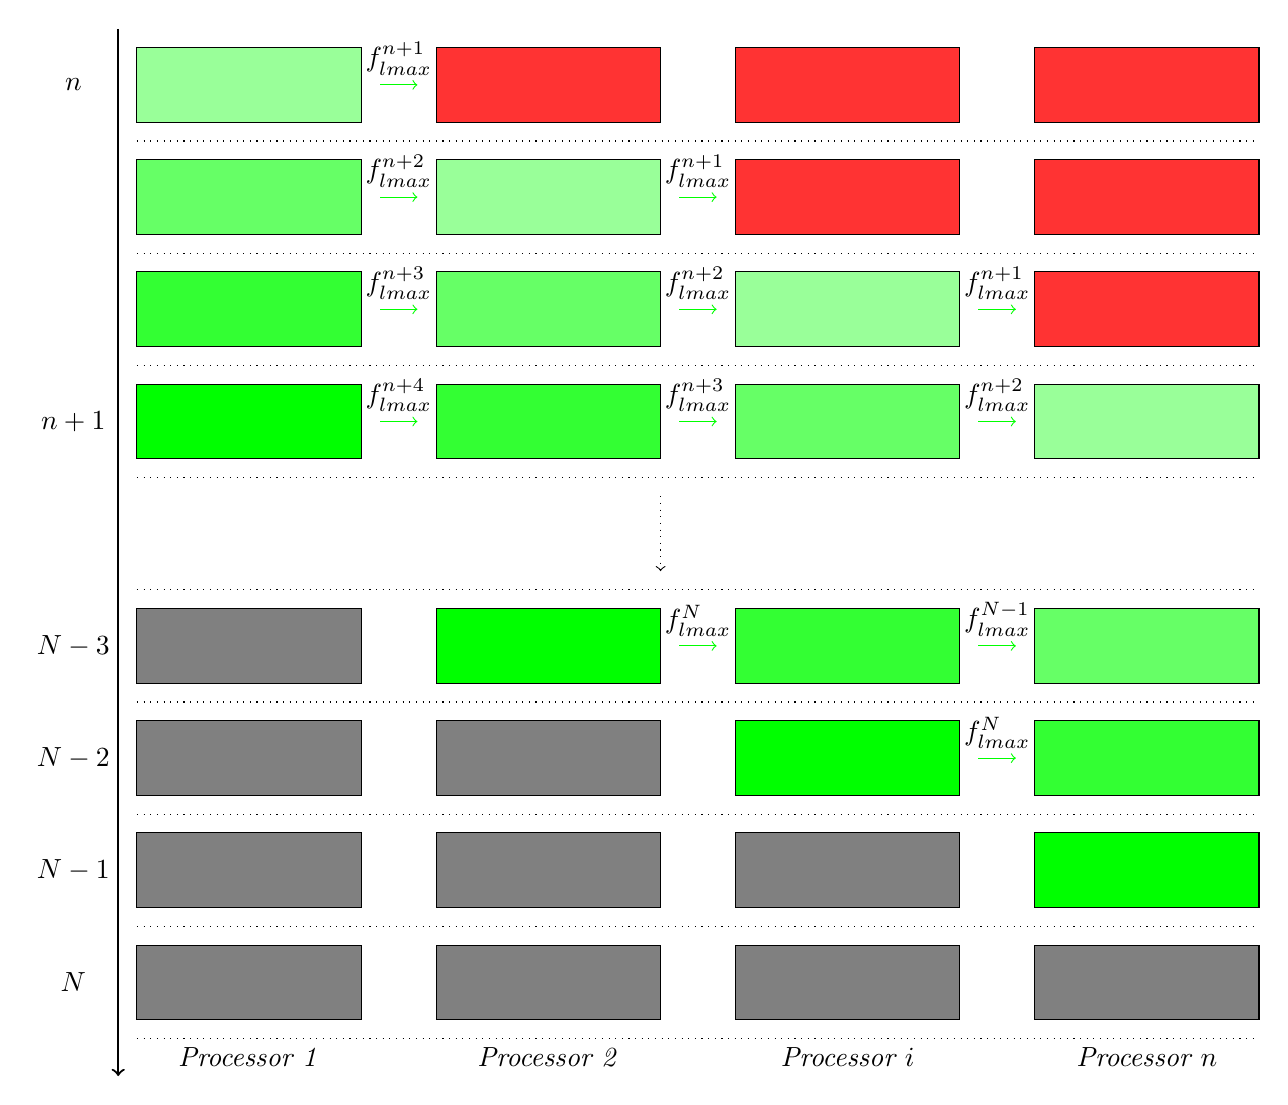
\begin{tikzpicture}[scale=0.95]
			\draw [->] [black, thick] (-.25, 0.25) -- (-.25, -13.75);
			\node[black] at (-0.85, -0.5) {$n$};
			\draw [->][green] (3.25, -0.5) -- node [midway, above, sloped, black] {$f_{lmax}^{n+1}$} (3.75, -.5);
			\filldraw[fill=green!40!white, draw=black] (0,0) rectangle (3,-1);
			\filldraw[fill=red!80!white, draw=black] (4,0) rectangle (7,-1);
			\filldraw[fill=red!80!white, draw=black] (8,0) rectangle (11,-1);
			\filldraw[fill=red!80!white, draw=black] (12,0) rectangle (15,-1);
			\draw [dotted] (0,-1.25) -- (15,-1.25);
			
			\draw [->][green] (3.25, -2) -- node [midway, above, sloped, black] {$f_{lmax}^{n+2}$} (3.75, -2);
			\draw [->][green] (7.25, -2) -- node [midway, above, sloped, black] {$f_{lmax}^{n+1}$} (7.75, -2);
			\filldraw[fill=green!60!white, draw=black] (0,-1.5) rectangle (3,-2.5);
			\filldraw[fill=green!40!white, draw=black] (4,-1.5) rectangle (7,-2.5);
			\filldraw[fill=red!80!white, draw=black] (8,-1.5) rectangle (11,-2.5);
			\filldraw[fill=red!80!white, draw=black] (12,-1.5) rectangle (15,-2.5);
			\draw [dotted] (0,-2.75) -- (15,-2.75);
			
			\draw [->][green] (3.25, -3.5) -- node [midway, above, sloped, black] {$f_{lmax}^{n+3}$} (3.75, -3.5);
			\draw [->][green] (7.25, -3.5) -- node [midway, above, sloped, black] {$f_{lmax}^{n+2}$} (7.75, -3.5);
			\draw [->][green] (11.25, -3.5) -- node [midway, above, sloped, black] {$f_{lmax}^{n+1}$} (11.75, -3.5);
			\filldraw[fill=green!80!white, draw=black] (0,-3) rectangle (3,-4);
			\filldraw[fill=green!60!white, draw=black] (4,-3) rectangle (7,-4);
			\filldraw[fill=green!40!white, draw=black] (8,-3) rectangle (11,-4);
			\filldraw[fill=red!80!white, draw=black] (12,-3) rectangle (15,-4);
			\draw [dotted] (0,-4.25) -- (15,-4.25);
			
			\node[black] at (-0.85, -5) {$n+1$};
			\draw [->][green] (3.25, -5) -- node [midway, above, sloped, black] {$f_{lmax}^{n+4}$} (3.75, -5);
			\draw [->][green] (7.25, -5) -- node [midway, above, sloped, black] {$f_{lmax}^{n+3}$} (7.75, -5);
			\draw [->][green] (11.25, -5) -- node [midway, above, sloped, black] {$f_{lmax}^{n+2}$} (11.75, -5);
			\filldraw[fill=green!100!white, draw=black] (0,-4.5) rectangle (3,-5.5);
			\filldraw[fill=green!80!white, draw=black] (4,-4.5) rectangle (7,-5.5);
			\filldraw[fill=green!60!white, draw=black] (8,-4.5) rectangle (11,-5.5);
			\filldraw[fill=green!40!white, draw=black] (12,-4.5) rectangle (15,-5.5);
			\draw [dotted] (0,-5.75) -- (15,-5.75);
			
			\draw [->][dotted] (7,-6) -- (7,-7);
			\draw [dotted] (0,-7.25) -- (15,-7.25);	
			
			\node[black] at (-0.85, -8) {$N-3$};
			\draw [->][green] (7.25, -8) -- node [midway, above, sloped, black] {$f_{lmax}^{N}$} (7.75, -8);
			\draw [->][green] (11.25, -8) -- node [midway, above, sloped, black] {$f_{lmax}^{N-1}$} (11.75, -8);
			\filldraw[fill=gray!100!white, draw=black] (0,-7.5) rectangle (3,-8.5);
			\filldraw[fill=green!100!white, draw=black] (4,-7.5) rectangle (7,-8.5);
			\filldraw[fill=green!80!white, draw=black] (8,-7.5) rectangle (11,-8.5);
			\filldraw[fill=green!60!white, draw=black] (12,-7.5) rectangle (15,-8.5);
			\draw [dotted] (0,-8.75) -- (15,-8.75);
			
			\node[black] at (-0.85, -9.5) {$N-2$};
			\draw [->][green] (11.25, -9.5) -- node [midway, above, sloped, black] {$f_{lmax}^{N}$} (11.75, -9.5);
			\filldraw[fill=gray!100!white, draw=black] (0,-9) rectangle (3,-10);
			\filldraw[fill=gray!100!white, draw=black] (4,-9) rectangle (7,-10);
			\filldraw[fill=green!100!white, draw=black] (8,-9) rectangle (11,-10);
			\filldraw[fill=green!80!white, draw=black] (12,-9) rectangle (15,-10);
			\draw [dotted] (0,-10.25) -- (15,-10.25);
			
			\node[black] at (-0.85, -11) {$N-1$};
			\filldraw[fill=gray!100!white, draw=black] (0,-10.5) rectangle (3,-11.5);
			\filldraw[fill=gray!100!white, draw=black] (4,-10.5) rectangle (7,-11.5);
			\filldraw[fill=gray!100!white, draw=black] (8,-10.5) rectangle (11,-11.5);
			\filldraw[fill=green!1000!white, draw=black] (12,-10.5) rectangle (15,-11.5);
			\draw [dotted] (0,-11.75) -- (15,-11.75);
			
			\node[black] at (-0.85, -12.5) {$N$};
			\filldraw[fill=gray!100!white, draw=black] (0,-12) rectangle (3,-13);
			\filldraw[fill=gray!100!white, draw=black] (4,-12) rectangle (7,-13);
			\filldraw[fill=gray!100!white, draw=black] (8,-12) rectangle (11,-13);
			\filldraw[fill=gray!100!white, draw=black] (12,-12) rectangle (15,-13);
			\draw [dotted] (0,-13.25) -- (15,-13.25);
			
			\node[align=right] at (1.5, -13.5) {\emph{Processor 1}};
			\node[align=right] at (5.5, -13.5) {\emph{Processor 2}};
			\node[align=right] at (9.5, -13.5) {\emph{Processor $i$}};
			\node[align=right] at (13.5, -13.5) {\emph{Processor $n$}};
		
		\end{tikzpicture}
		\caption{Visualization of parallel calculations for implicit upwind scheme for $\gls{CFL} > 0$.}
		\label{fig:visualization:implicit-upwind}
	\end{figure}
	If $N$ is a number of iterations in a time domain and $n$ is number of processors then a total time spent on waiting for new data between processors is equal to $n$. Thus calculations are performed simultaneously for $N - n$ unit times. Left axis of Figure \ref{fig:visualization:implicit-upwind} relates to finished iteration on entire grid.
	\subsection{Crank--Nicolson scheme parallel algorithm} \label{s:general-approach:crank-nicolson-parallel-algorithm}
	Crank--Nicolson numerical methods is an implicit scheme, which requires to solve a matrix to get new solution at time step $n+1$. According to formula \eqref{eq:crani-nicolson:matrix} we can see that matrix $A$ is tridiagonal. George Em Karniadakis and Robert M. Kirby II in \cite{bib:mpi}[p. 359 -- 361] proposed \emph{Thomas Algorithm for Tridiagonal Systems}. Mentioned algorithm has three stages:
	\begin{enumerate}
		\item (LU Decomposition) $A = LU$;
		\item (Forward Substitution) $Ly = q$;
		\item (Backward Substitution) $Ux = y$
	\end{enumerate}
	Unfortunately backward and forward substitutions have dependency to previous and next element respectively. It means that there is no way to speedup those stages using parallel approach. The only way to improve performance of Thomas algorithm in terms of Crank-Nicolson scheme is to make use of a fact that tridiagonal dominant matrix will have the same values of element for every iterations -- it can be calculated at the beginning only once during initialization of dependent variables shown in Figure \ref{fig:schematicOfFDM}.
	\begin{figure}[!htbp]
		\centering
		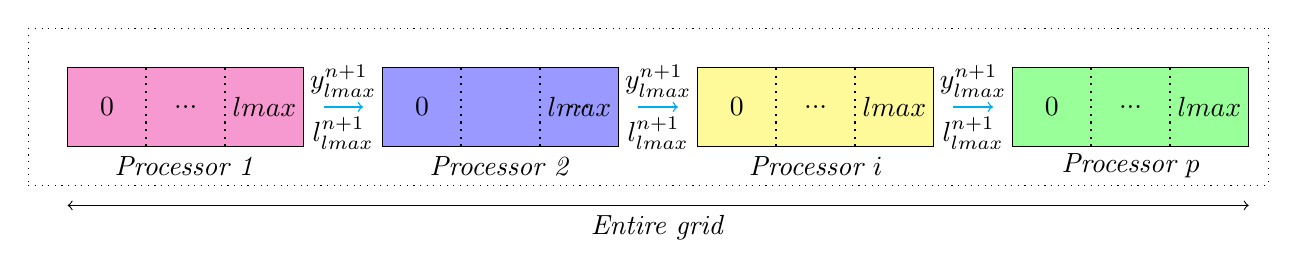
\begin{tikzpicture}[scale=1.0]
			\draw[dotted] (-0.5,-0.5) -- (15.25,-0.5);
			\draw[dotted] (-0.5, 1.5) -- (15.25, 1.5);
			\draw[dotted] (-0.5, 1.5) -- (-0.5, -0.5);
			\draw[dotted] (15.25, 1.5) -- (15.25, -0.5);
			
			\filldraw[fill=magenta!40!white, draw=black] (0,0) rectangle (3,1);
			\node[black] at (0.5,0.5) {$0$};
			\draw[black, dotted, line width = 0.75pt] (1, 0) -- (1, 1);
			\node[black] at (1.5,0.5) {...};
			\draw[black, dotted, line width = 0.75pt] (2, 0) -- (2, 1);
			\node[black] at (2.5,0.5) {$lmax$};
			
			\filldraw[fill=blue!40!white, draw=black] (4,0) rectangle (7,1);
			\node[black] at (4.5,0.5) {$0$};
			\draw[black, dotted, line width = 0.75pt] (5, 0) -- (5, 1);
			\node[black] at (6.5,0.5) {...};
			\draw[black, dotted, line width = 0.75pt] (6, 0) -- (6, 1);
			\node[black] at (6.5,0.5) {$lmax$};
			
			\filldraw[fill=yellow!40!white, draw=black] (8,0) rectangle (11,1);
			\node[black] at (8.5,0.5) {$0$};
			\draw[black, dotted, line width = 0.75pt] (9, 0) -- (9, 1);
			\node[black] at (9.5,0.5) {...};
			\draw[black, dotted, line width = 0.75pt] (10, 0) -- (10, 1);
			\node[black] at (10.5,0.5) {$lmax$};
			
			\filldraw[fill=green!40!white, draw=black] (12,0) rectangle (15,1);
			\node[black] at (12.5,0.5) {$0$};
			\draw[black, dotted, line width = 0.75pt] (13, 0) -- (13, 1);
			\node[black] at (13.5,0.5) {...};
			\draw[black, dotted, line width = 0.75pt] (14, 0) -- (14, 1);
			\node[black] at (14.5,0.5) {$lmax$};
			
			\node[align=right] at (1.5, -0.25) {\emph{Processor 1}};
			\node[align=right] at (5.5, -0.25) {\emph{Processor 2}};
			\node[align=right] at (9.5, -0.25) {\emph{Processor $i$}};
			\node[align=right] at (13.5, -0.25) {\emph{Processor $p$}};
			\draw [->][cyan] (3.25, 0.5) -- node [midway, above, sloped, black] {$y_{lmax}^{n+1}$} (3.75, 0.5);
			\draw [->][cyan] (7.25, 0.5) -- node [midway, above, sloped, black] {$y_{lmax}^{n+1}$} (7.75, 0.5);
			\draw [->][cyan] (11.25, 0.5) -- node [midway, above, sloped, black] {$y_{lmax}^{n+1}$} (11.75, 0.5);
			\draw [->][cyan] (3.25, 0.5) -- node [midway, below, sloped, black] {$l_{lmax}^{n+1}$} (3.75, 0.5);
			\draw [->][cyan] (7.25, 0.5) -- node [midway, below, sloped, black] {$l_{lmax}^{n+1}$} (7.75, 0.5);
			\draw [->][cyan] (11.25, 0.5) -- node [midway, below, sloped, black] {$l_{lmax}^{n+1}$} (11.75, 0.5);
			\draw[<->] (0,-0.75) -- node [midway, below, sloped, black] {\emph{Entire grid}} (15,-0.75);
		\end{tikzpicture}
		\caption{Communication between processors during forward substitution.}
		\label{fig:communication:forward-substitution}
	\end{figure}
	In a serial way backward and forward substitutions requires an entire grid and dependent LU decomposition matrices. Using this approach main processor would need to gather all local grids from the processors, which later would be used in a serial algorithm. Moreover after this it would required to scatter new solution to processors, which highly increases the load of communication without increase of efficiency. Due to that remark it would be better to make use of a serial Thomas algorithm in a way that communication between processors stays as low as possible. Mentioned in Section \ref{s:general-approach:devise-a-way-to-parallelize} spreading grid across all processors is a good idea.
	\begin{figure}[!htbp]
		\centering
		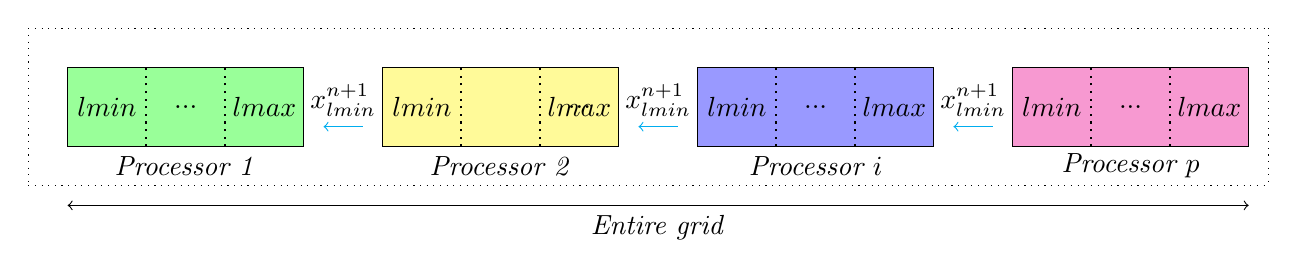
\begin{tikzpicture}[scale=1.0]
			\draw[dotted] (-0.5,-0.5) -- (15.25,-0.5);
			\draw[dotted] (-0.5, 1.5) -- (15.25, 1.5);
			\draw[dotted] (-0.5, 1.5) -- (-0.5, -0.5);
			\draw[dotted] (15.25, 1.5) -- (15.25, -0.5);
			\filldraw[fill=green!40!white, draw=black] (0,0) rectangle (3,1);
			\node[black] at (0.5,0.5) {$lmin$};
			\draw[black, dotted, line width = 0.75pt] (1, 0) -- (1, 1);
			\node[black] at (1.5,0.5) {...};
			\draw[black, dotted, line width = 0.75pt] (2, 0) -- (2, 1);
			\node[black] at (2.5,0.5) {$lmax$};
			
			\filldraw[fill=yellow!40!white, draw=black] (4,0) rectangle (7,1);
			\node[black] at (4.5,0.5) {$lmin$};
			\draw[black, dotted, line width = 0.75pt] (5, 0) -- (5, 1);
			\node[black] at (6.5,0.5) {...};
			\draw[black, dotted, line width = 0.75pt] (6, 0) -- (6, 1);
			\node[black] at (6.5,0.5) {$lmax$};
			
			\filldraw[fill=blue!40!white, draw=black] (8,0) rectangle (11,1);
			\node[black] at (8.5,0.5) {$lmin$};
			\draw[black, dotted, line width = 0.75pt] (9, 0) -- (9, 1);
			\node[black] at (9.5,0.5) {...};
			\draw[black, dotted, line width = 0.75pt] (10, 0) -- (10, 1);
			\node[black] at (10.5,0.5) {$lmax$};
			
			\filldraw[fill=magenta!40!white, draw=black] (12,0) rectangle (15,1);
			\node[black] at (12.5,0.5) {$lmin$};
			\draw[black, dotted, line width = 0.75pt] (13, 0) -- (13, 1);
			\node[black] at (13.5,0.5) {...};
			\draw[black, dotted, line width = 0.75pt] (14, 0) -- (14, 1);
			\node[black] at (14.5,0.5) {$lmax$};
			
			\node[align=right] at (1.5, -0.25) {\emph{Processor 1}};
			\node[align=right] at (5.5, -0.25) {\emph{Processor 2}};
			\node[align=right] at (9.5, -0.25) {\emph{Processor $i$}};
			\node[align=right] at (13.5, -0.25) {\emph{Processor $p$}};
			\draw [<-][cyan] (3.25, 0.25) -- node [midway, above, sloped, black] {$x_{lmin}^{n+1}$} (3.75, 0.25);
			\draw [<-][cyan] (7.25, 0.25) -- node [midway, above, sloped, black] {$x_{lmin}^{n+1}$} (7.75, 0.25);
			\draw [<-][cyan] (11.25, 0.25) -- node [midway, above, sloped, black] {$x_{lmin}^{n+1}$} (11.75, 0.25);
			\draw[<->] (0,-0.75) -- node [midway, below, sloped, black] {\emph{Entire grid}} (15,-0.75);
		\end{tikzpicture}
		\caption{Communication between processors during backward substitution.}
		\label{fig:communication:backward-substitution}
	\end{figure}
	During processing second and third stage of Thomas algorithm each processor will require to send/receive only 2 values in case of forward substitution and one for backward. So the value of communication decreased from double grid size to triple amount of processors. It is very likely that quantity of processors is much lower than size of the grid, thus this approach is valid.
	
	Looking at right side of Equation \eqref{eq:crani-nicolson:matrix}, dependencies \eqref{eq:crank-nicolson:dependencies-matrix} and \gls{stencil} \ref{fig:stencil:crank-nicolson} we observe that current solution depends on the left and right point at time $n$. It is possible to conclude two conclusions: processors will be able to work simultaneously after exchanging two boundaries from neighboring processors, although still solving of tridiagonal dominant matrix will be required to solve after. Due to idea of spreading grid locally we can prove its even better idea to keep data locally rather than exchanging entire grid in order to invoke Thomas algorithm.	
	\begin{figure}[!htbp]
		\centering
		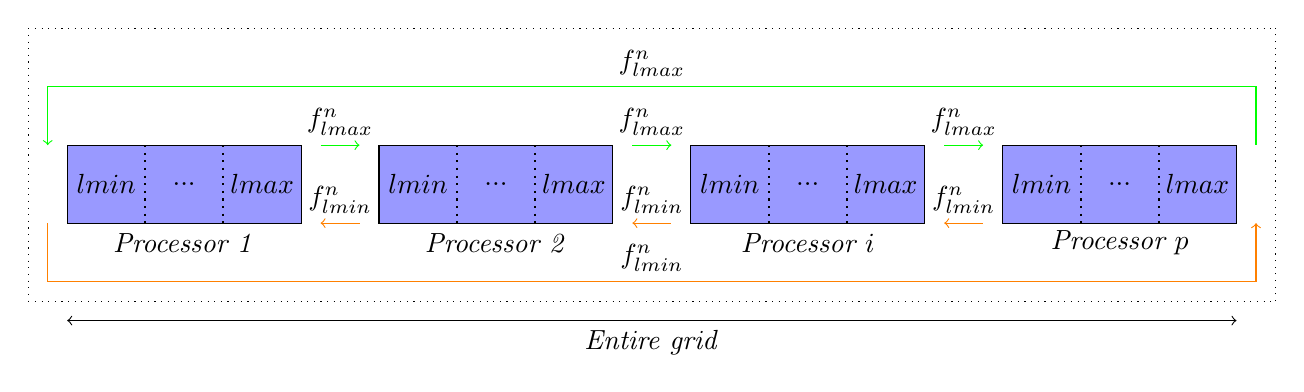
\begin{tikzpicture}[scale=0.99]
			\draw[dotted] (-0.5,1.5) -- (15.5,1.5);
			\draw[dotted] (-0.5, -2) -- (15.5, -2);
			\draw[dotted] (-0.5, 1.5) -- (-0.5, -2);
			\draw[dotted] (15.5, -2) -- (15.5, 1.5);
			
			\filldraw[fill=blue!40!white, draw=black] (0,0) rectangle (3,-1);
			\node[black] at (0.5,-0.5) {$lmin$};
			\draw[black, dotted, line width = 0.75pt] (1, 0) -- (1, -1);
			\node[black] at (1.5,-0.5) {...};
			\draw[black, dotted, line width = 0.75pt] (2, 0) -- (2, -1);
			\node[black] at (2.5,-0.5) {$lmax$};
			
			\filldraw[fill=blue!40!white, draw=black] (4,0) rectangle (7,-1);
			\node[black] at (4.5,-0.5) {$lmin$};
			\draw[black, dotted, line width = 0.75pt] (5, 0) -- (5, -1);
			\node[black] at (5.5,-0.5) {...};
			\draw[black, dotted, line width = 0.75pt] (6, 0) -- (6, -1);
			\node[black] at (6.5,-0.5) {$lmax$};
			
			\filldraw[fill=blue!40!white, draw=black] (8,0) rectangle (11,-1);
			\node[black] at (8.5,-0.5) {$lmin$};
			\draw[black, dotted, line width = 0.75pt] (9, 0) -- (9, -1);
			\node[black] at (9.5,-0.5) {...};
			\draw[black, dotted, line width = 0.75pt] (10, 0) -- (10, -1);
			\node[black] at (10.5,-0.5) {$lmax$};
			
			\filldraw[fill=blue!40!white, draw=black] (12,0) rectangle (15,-1);
			\node[black] at (12.5,-0.5) {$lmin$};
			\draw[black, dotted, line width = 0.75pt] (13, 0) -- (13, -1);
			\node[black] at (13.5,-0.5) {...};
			\draw[black, dotted, line width = 0.75pt] (14, 0) -- (14, -1);
			\node[black] at (14.5,-0.5) {$lmax$};
			
			
			\node[align=right] at (1.5, -1.25) {\emph{Processor 1}};
			\node[align=right] at (5.5, -1.25) {\emph{Processor 2}};
			\node[align=right] at (9.5, -1.25) {\emph{Processor $i$}};
			\node[align=right] at (13.5, -1.25) {\emph{Processor $p$}};
			
			\draw [->][green] (3.25, 0) -- node [midway, above, sloped, black] {$f_{lmax}^{n}$} (3.75, 0);
			\draw [->][green] (7.25, 0) -- node [midway, above, sloped, black] {$f_{lmax}^{n}$} (7.75, 0);
			\draw [->][green] (11.25, 0) -- node [midway, above, sloped, black] {$f_{lmax}^{n}$} (11.75, 0);
			
			
			\draw [<-][orange] (3.25, -1) -- node [midway, above, sloped, black] {$f_{lmin}^{n}$} (3.75, -1);
			\draw [<-][orange] (7.25, -1) -- node [midway, above, sloped, black] {$f_{lmin}^{n}$} (7.75, -1);
			\draw [<-][orange] (11.25, -1) -- node [midway, above, sloped, black] {$f_{lmin}^{n}$} (11.75, -1);
			
			\draw [<-][green] (-.25, 0) -- (-.25, 0.75) -- node [midway, above, sloped, black] {$f_{lmax}^{n}$} (15.25, 0.75) -- (15.25, 0);
			
			\draw [->][orange] (-.25, -1) -- (-.25, -1.75) -- node [midway, above, sloped, black] {$f_{lmin}^{n}$} (15.25, -1.75) -- (15.25, -1);
			
			\draw[<->] (0,-2.25) -- node [midway, below, sloped, black] {\emph{Entire grid}} (15,-2.25);
		\end{tikzpicture}
		\caption{Communication between processors in parallel Crank-Nicolson schema.}
		\label{fig:communication:crank-nicolson}
	\end{figure}
	Figure \ref{fig:communication:crank-nicolson} presents communication in parallel Crank-Nicolson numerical schema. It is clearly visible that each processor has to exchange two values. In case of backward (Figure \ref{fig:communication:backward-substitution}) and forward (Figure \ref{fig:communication:forward-substitution}) substitution only one value is send between processors starting from respectively last and first processor.
	\begin{figure}[!htbp]
		\centering
		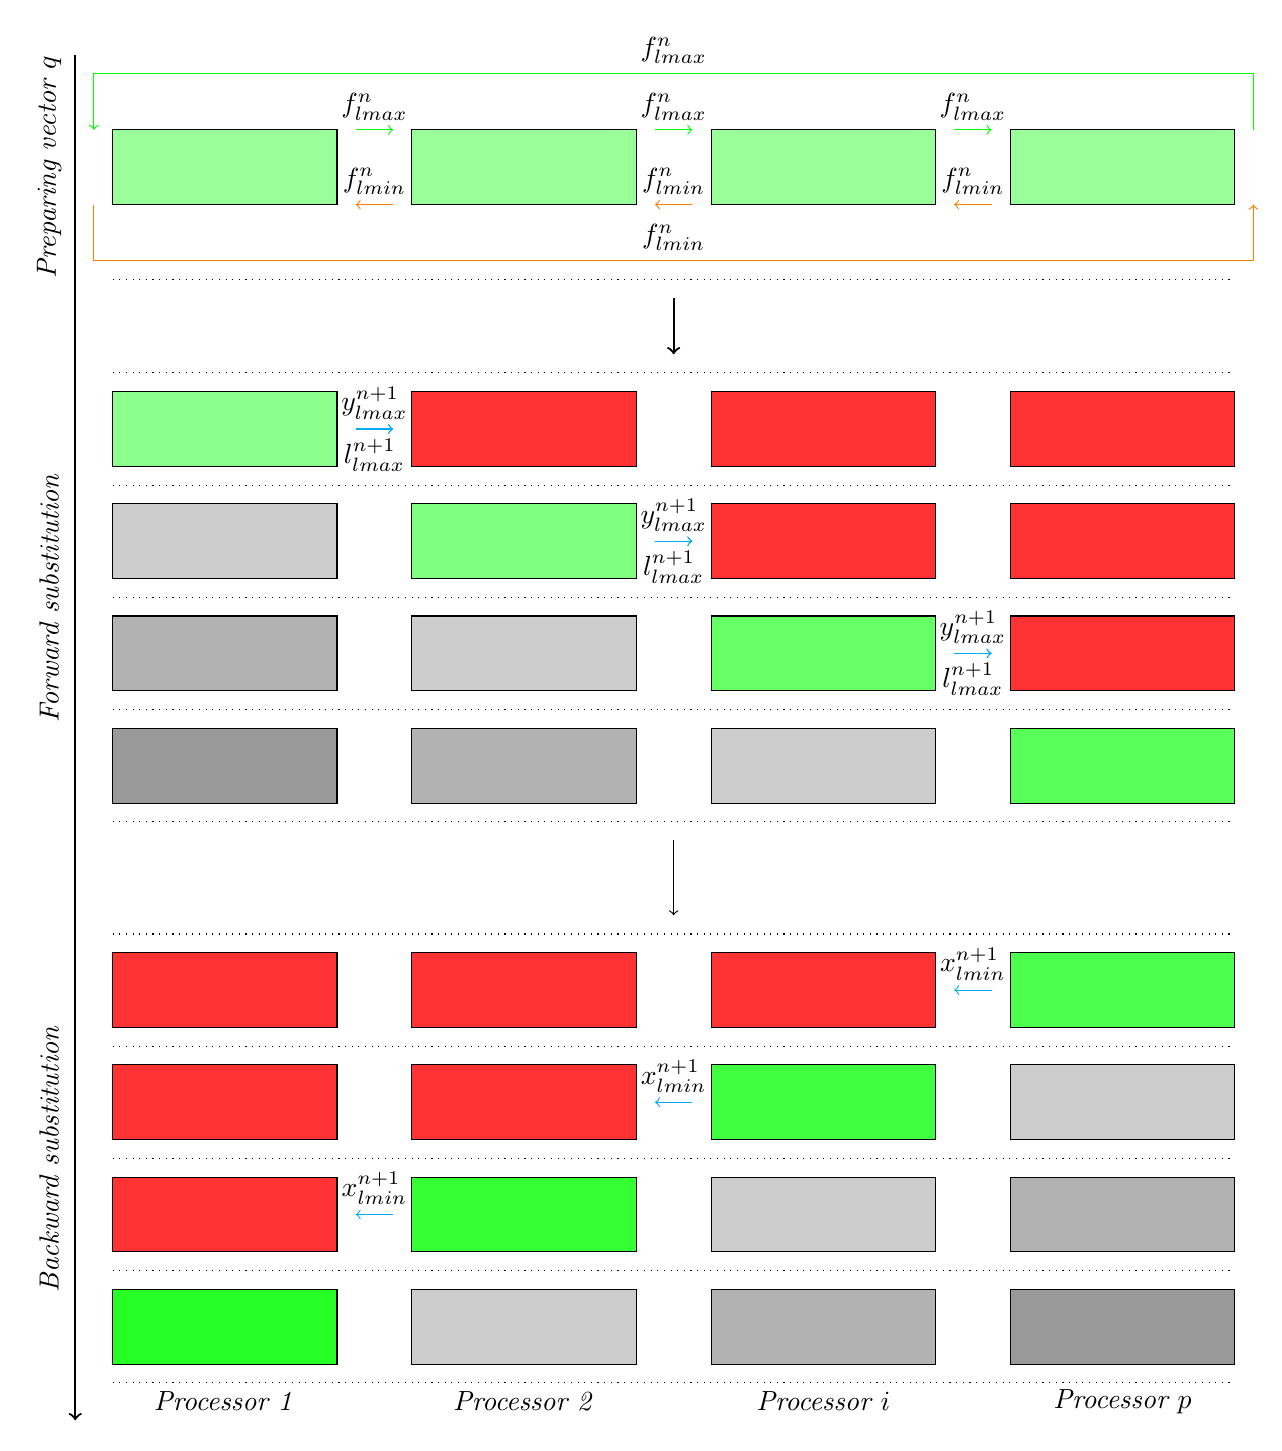
\begin{tikzpicture}[scale=0.95]
			\draw [->] [black, thick] (-.5, 4.5) -- (-.5, -13.75);
			
			\node[black] at (-0.85, 3) {\rotatebox{90}{\emph{Preparing vector $q$}}};
			\filldraw[fill=green!40!white, draw=black] (0, 3.5) rectangle (3, 2.5);
			\filldraw[fill=green!40!white, draw=black] (4, 3.5) rectangle (7, 2.5);
			\filldraw[fill=green!40!white, draw=black] (8, 3.5) rectangle (11, 2.5);
			\filldraw[fill=green!40!white, draw=black] (12, 3.5) rectangle (15, 2.5);
			\draw [->][green] (3.25, 3.5) -- node [midway, above, sloped, black] {$f_{lmax}^{n}$} (3.75, 3.5);
			\draw [->][green] (7.25, 3.5) -- node [midway, above, sloped, black] {$f_{lmax}^{n}$} (7.75, 3.5);
			\draw [->][green] (11.25, 3.5) -- node [midway, above, sloped, black] {$f_{lmax}^{n}$} (11.75, 3.5);	
			\draw [<-][orange] (3.25, 2.5) -- node [midway, above, sloped, black] {$f_{lmin}^{n}$} (3.75, 2.5);
			\draw [<-][orange] (7.25, 2.5) -- node [midway, above, sloped, black] {$f_{lmin}^{n}$} (7.75, 2.5);
			\draw [<-][orange] (11.25, 2.5) -- node [midway, above, sloped, black] {$f_{lmin}^{n}$} (11.75, 2.5);	
			\draw [<-][green] (-.25, 3.5) -- (-.25, 4.25) -- node [midway, above, sloped, black] {$f_{lmax}^{n}$} (15.25, 4.25) -- (15.25, 3.5);		
			\draw [->][orange] (-.25, 2.5) -- (-.25, 1.75) -- node [midway, above, sloped, black] {$f_{lmin}^{n}$} (15.25, 1.75) -- (15.25, 2.5);	
			
			\draw [dotted] (0, 1.5) -- (15, 1.5);
			\draw [->] [black, thick] (7.5, 1.25) -- (7.5, .5);
			\draw [dotted] (0, .25) -- (15, .25);
			
			\node[black] at (-0.85, -2.75) {\rotatebox{90}{\emph{Forward substitution}}};
			\draw [->][cyan] (3.25, -0.5) -- node [midway, above, sloped, black] {$y_{lmax}^{n+1}$} (3.75, -.5);
			\draw [->][cyan] (3.25, -0.5) -- node [midway, below, sloped, black] {$l_{lmax}^{n+1}$} (3.75, -.5);
			\filldraw[fill=green!45!white, draw=black] (0,0) rectangle (3,-1);
			\filldraw[fill=red!80!white, draw=black] (4,0) rectangle (7,-1);
			\filldraw[fill=red!80!white, draw=black] (8,0) rectangle (11,-1);
			\filldraw[fill=red!80!white, draw=black] (12,0) rectangle (15,-1);
			\draw [dotted] (0,-1.25) -- (15,-1.25);
			
			\draw [->][cyan] (7.25, -2) -- node [midway, above, sloped, black] {$y_{lmax}^{n+1}$} (7.75, -2);
			\draw [->][cyan] (7.25, -2) -- node [midway, below, sloped, black] {$l_{lmax}^{n+1}$} (7.75, -2);
			\filldraw[fill=gray!40!white, draw=black] (0,-1.5) rectangle (3,-2.5);
			\filldraw[fill=green!50!white, draw=black] (4,-1.5) rectangle (7,-2.5);
			\filldraw[fill=red!80!white, draw=black] (8,-1.5) rectangle (11,-2.5);
			\filldraw[fill=red!80!white, draw=black] (12,-1.5) rectangle (15,-2.5);
			\draw [dotted] (0,-2.75) -- (15,-2.75);
			
			\draw [->][cyan] (11.25, -3.5) -- node [midway, above, sloped, black] {$y_{lmax}^{n+1}$} (11.75, -3.5);
			\draw [->][cyan] (11.25, -3.5) -- node [midway, below, sloped, black] {$l_{lmax}^{n+1}$} (11.75, -3.5);
			\filldraw[fill=gray!60!white, draw=black] (0,-3) rectangle (3,-4);
			\filldraw[fill=gray!40!white, draw=black] (4,-3) rectangle (7,-4);
			\filldraw[fill=green!60!white, draw=black] (8,-3) rectangle (11,-4);
			\filldraw[fill=red!80!white, draw=black] (12,-3) rectangle (15,-4);
			\draw [dotted] (0,-4.25) -- (15,-4.25);
			
			\filldraw[fill=gray!80!white, draw=black] (0,-4.5) rectangle (3,-5.5);
			\filldraw[fill=gray!60!white, draw=black] (4,-4.5) rectangle (7,-5.5);
			\filldraw[fill=gray!40!white, draw=black] (8,-4.5) rectangle (11,-5.5);
			\filldraw[fill=green!65!white, draw=black] (12,-4.5) rectangle (15,-5.5);
			\draw [dotted] (0,-5.75) -- (15,-5.75);
			
			\draw [->][black] (7.5,-6) -- (7.5,-7);
			\draw [dotted] (0,-7.25) -- (15,-7.25);	
			
			\node[black] at (-0.85, -10.25) {\rotatebox{90}{\emph{Backward substitution}}};
			\draw [->][cyan] (11.75, -8) -- node [midway, above, sloped, black] {$x_{lmin}^{n+1}$} (11.25, -8);
			\filldraw[fill=red!80!white, draw=black] (0,-7.5) rectangle (3,-8.5);
			\filldraw[fill=red!80!white, draw=black] (4,-7.5) rectangle (7,-8.5);
			\filldraw[fill=red!80!white, draw=black] (8,-7.5) rectangle (11,-8.5);
			\filldraw[fill=green!70!white, draw=black] (12,-7.5) rectangle (15,-8.5);
			\draw [dotted] (0,-8.75) -- (15,-8.75);
			
			\draw [->][cyan] (7.75, -9.5) -- node [midway, above, sloped, black] {$x_{lmin}^{n+1}$} (7.25, -9.5);
			\filldraw[fill=red!80!white, draw=black] (0,-9) rectangle (3,-10);
			\filldraw[fill=red!80!white, draw=black] (4,-9) rectangle (7,-10);
			\filldraw[fill=green!75!white, draw=black] (8,-9) rectangle (11,-10);
			\filldraw[fill=gray!40!white, draw=black] (12,-9) rectangle (15,-10);
			\draw [dotted] (0,-10.25) -- (15,-10.25);
			
			\draw [->][cyan] (3.75, -11) -- node [midway, above, sloped, black] {$x_{lmin}^{n+1}$} (3.25, -11);
			\filldraw[fill=red!80!white, draw=black] (0,-10.5) rectangle (3,-11.5);
			\filldraw[fill=green!80!white, draw=black] (4,-10.5) rectangle (7,-11.5);
			\filldraw[fill=gray!40!white, draw=black] (8,-10.5) rectangle (11,-11.5);
			\filldraw[fill=gray!60!white, draw=black] (12,-10.5) rectangle (15,-11.5);
			\draw [dotted] (0,-11.75) -- (15,-11.75);
			
			\filldraw[fill=green!85!white, draw=black] (0,-12) rectangle (3,-13);
			\filldraw[fill=gray!40!white, draw=black] (4,-12) rectangle (7,-13);
			\filldraw[fill=gray!60!white, draw=black] (8,-12) rectangle (11,-13);
			\filldraw[fill=gray!80!white, draw=black] (12,-12) rectangle (15,-13);
			\draw [dotted] (0,-13.25) -- (15,-13.25);
			
			\node[align=right] at (1.5, -13.5) {\emph{Processor 1}};
			\node[align=right] at (5.5, -13.5) {\emph{Processor 2}};
			\node[align=right] at (9.5, -13.5) {\emph{Processor $i$}};
			\node[align=right] at (13.5, -13.5) {\emph{Processor $p$}};
			
		\end{tikzpicture}
		\caption{Visualization of parallel calculations for Crank-Nicolson scheme.}
		\label{fig:visualization:crank-nicolson}
	\end{figure}
	Presented communication in Figure \ref{fig:visualization:crank-nicolson} shows a process of acquiring new solution. This schematic does not contain initialization of matrices $l$, $u$, $d$, which are similarly to implicit upwind scheme created at the beginning of discretization process as mentioned before in \ref{s:general-approach:implicit-upwind-parallel-algorithm}.
	\clearpage